\chapter{Introdução}
A Diabetes Melito é uma doença que surge quando o organismo deixa de produzir insulina ou quando a essa passa a não atuar com a mesma eficácia. Atualmente existe duas classificações para ela: Diabetes Melito tipo 1 e 2. A primeira se caracteriza por ser autoimune que lesa, de forma irreversível, as células do pâncreas, produtoras de insulina e conhecidas como células beta, e seu diagnóstico se dá durante a infância do portador. Enquanto a segunda é consequência da resistência do próprio organismo contra as ações da insulina, o principal fator para se desenvolver essa resistência é a obesidade\cite{portaldiabetes2008}.
Bomba de infusão de insulina é um pequeno aparelho eletrônico, do tamanho de um celular ou pager, que está ligado ao corpo do portador da doença por um finíssimo cateter com uma agulha flexível na ponta. Essa agulha é inserida no braço, coxa ou abdômen e deve ser trocada em um período de 2 ou 3 dias. Essa bomba não mede o índice glicêmico ou a quantidade de insulina a ser utilizada, essa medição é feita através do glicosímetro. A Figura ~\ref{fig:bombainfusao}\footnote{\url{http://www.diabetes.org.br/sala-de-noticias/2316-bombas-de-infusao-de-insulina}} representa um aparelho comercial.

\begin{figure}[htp]
	\centering
	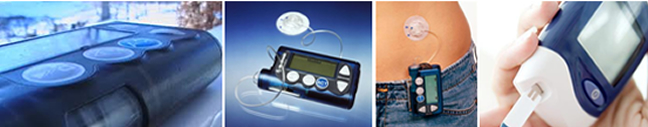
\includegraphics[scale=1]{images/bombainsulina.png}
	\caption{Imagens de uma bomba de infusão de insulina}	
	\label{fig:bombainfusao}	
\end{figure}


Seu funcionamento é bem simples, libera-se uma quantidade de insulina, programada pelo médico, durante o dia todo, simulando o funcionamento do pâncreas de uma pessoa saudável, entretanto existem cuidados a serem tomados: calcular a quantidade de carboidratos ingeridos a cada refeição e programar o aparelho para injetar uma quantidade de insulina com maior velocidade no organismo.
Quanto a quem pode usar, a pessoa deve cumprir alguns pré-requisitos que são:
\begin{itemize}
\item Conseguir medir o índice glicêmico no mínimo 4 vezes por dia;
\item Durante a fase de adaptação e ajuste da dosagem a serem utilizadas pela bomba, fazer a medição glicêmica de 6 a 8 vezes por dia;
\item Seguir as recomendações médicas além de manter contato e um constante \emph{feedback} com os responsáveis pela bomba e, além de tudo, seguir a dieta recomendada, respeitando quantidades ingeridas;
\item Ter condição financeira para custear o equipamento e o contato com os responsáveis por ele;
\item Estar disposto ao uso da bomba durante o dia todo, 24 horas junto ao corpo;
\item Aprender sobre contagem de carboidratos para saber seu consumo durante as refeições;
\item Praticar exercícios.
\end{itemize}

Cumprindo os pré-requisitos citados temos as vantagens de seu uso que são:

\begin{itemize}
\item Maior flexibilidade no horário das refeições;
\item Se usada corretamente o risco de hipoglicemia é reduzido, e a longo prazo as complicações devido ao diabetes também;
\item Melhora o controle glicêmico;
\item Melhora no controle do fenômeno do amanhecer, responsável pelo aumento do índice glicêmico durante a manha, entre as 4 e 8 horas da manha, causador da hipoglicemia se o diabético não calculou a dose de insulina antes de dormir, ou não se levantou durante a noite para gerenciá-la.
\end{itemize}

Mas mesmo com todas as vantagens dada devido ao uso do equipamento caso o diabético seja obeso, ingira grandes quantidades de alimento ou açúcar, ou seja, carboidratos, não praticar atividades físicas, não fazer a medição do índice glicêmico na quantidade de vezes recomendada, ou até mesmo determinar por si só a quantidade de insulina a ser utilizada, não existe vantagem no seu uso.
É importante ter em mente que mesmo com toda facilidade e tecnologia existente o acompanhamento médico não deve ser deixado de lado. As principais indicações médicas para o uso do equipamento são:

\begin{itemize}
\item Fenômeno do amanhecer;
\item Hipoglicemia;
\item Diminuir a variação do índice glicêmico;
\item Hiperglicemia;
\item Recorrente ceatosidade, que é o acumulo de ceatócidos, pois o fígado quebra a gordura e proteína devido à falta de insulina, pois o corpo não consegue utilizar a glicose como energia;
\item Flexibilidade, especialmente para crianças pequenas;
\item Gestação, viagens e atividade físicas;
\item Fobia de injeção;
\item Desejo do diabético \cite{diabetes2013, portaldiabetes2009}.
\end{itemize}

\section{Motivação}
Segundo a Sociedade Brasileira de Diabetes \cite{sbc2014}, diversos estudos realizados mostram que o tratamento feito através da Infusão de insulina tem diversas melhorias quando comparado com outros tratamentos existentes. Entretanto não é o mais utilizado devido ao seu alto custo, devido a importação.
Logo, esse projeto vem com foco social: facilitar o acesso da população brasileira de baixa renda ao equipamento, melhorando sua qualidade de vida dos portadores da doença que se encaixem nesse perfil. 

\section{OBJETIVOS}
Esse projeto tem como objetivo principal desenvolver um protótipo de uma Bomba de Infusão de insulina utilizando o microcontrolador da família PIC, PIC18F452. 

\subsection{OBJETIVOS SECUNDÀRIOS}

Em segundo plano este trabalho foca em:
\begin{itemize}
\item Aprendizado sobre as características e funcionalidades disponíveis do microcontrolador escolhido;
\item Aprendizado das tecnologias utilizadas como: compilador, simulador e bibliotecas disponíveis;
\item Desenvolvimento das funcionalidades básicas de uma bomba de infusão de insulina;
\item Aprendizado sobre a escolha e uso de um motor de passo;
\item Aprendizado sobre a forma de uso de um Display de LCD para comunicação com o usuário.
\end{itemize}

\section{PROCEDIMENTOS METODOLÓGICOS}
\todo{REVISAR QUANDO TERMINAR}\newline
Como todo trabalho de pesquisa, foi iniciado com o levantamento bibliográfico sobre o tema escolhido para que então seja feito uma leitura e análise desses materiais a fim de entender melhor sobre as dificuldades e possíveis formas de desenvolvimento. A elaboração da fundamentação teórica consiste nos assuntos: Microcontroladores – a base de nossa arquitetura e recursos de desenvolvimento –, PIC – plataforma escolhida para o desenvolvimento –, Motor de passo – responsável pela dinâmica da bomba –, e, por último, display de LCD – responsável por mostrar dados e estados da bomba em funcionamento.
Entendendo todos os conceitos citados o próximo passo deve ser a especificação do projeto de hardware do sistema embarcado, ou seja, qual placa usar, quais periféricos serão necessários, qual motor será utilizada, qual API do PIC utilizar. A simulação e desenvolvimento do hardware serão feitos na ferramenta Proteus, pois possui integração com PIC.
Tendo todo o hardware definido é necessário levantar os requisitos de software. Para entender o que deve ser desenvolvido e ter uma orientação do próprio desenvolvimento. Com os requisitos em mãos será possível definir a arquitetura do sistema. Para enfim dar inicio a implementação e testes do software. Quando ele tiver uma base concreta daremos inicio a integração com o hardware e validação de seu funcionamento. E por fim levantaremos os indicadores para que seja feita a comparação de desenvolvimento entre as plataformas citadas e poder concluir a pesquisa.
